%%%%%%%%%%%%%%%%%%%%%%%%%%%%%%%%%%%%%%%%%%%%%%%%%%%%%%%%%%%%%%%%%%%%%%%%%%%%%%%%
%%%                               80 COLONNES                                %%%
%%%%%%%%%%%%%%%%%%%%%%%%%%%%%%%%%%%%%%%%%%%%%%%%%%%%%%%%%%%%%%%%%%%%%%%%%%%%%%%%

\chapter{Contexte et problématique}
\label{ChCtxProb}

%%%%%%%%%%%%%%%%%%%%%%%%%%%%%%%%%%%%%%%%%%%%%%%%%%%%%%%%%%%%%%%%%%%%%%%%%%%%%

\section{Réseaux de capteurs et actionneurs sans-fil}
\label{SecWSN}


\subsection[Définitions]{Définitions~: technologie des réseaux de capteurs
                         et actionneurs sans-fil}
\label{SubsecDefWSN}

Les avancées spectaculaires des dernières décennies en micro-électronique,
notamment dans la domaine de la miniaturisation, de l'augmentation constante
de la puissance des circuits intégrés, ainsi que dans le domaine de la
communication sans-fil~--- principalement par des moyens radio~--- ont permis
l'émergence d'appareils électroniques miniatures (Microsystèmes
électromécaniques~: MEMS) capables d'interagir avec leur environnement
physique, de traiter des données et de communiquer entre eux et avec d'autres
systèmes informatiques sans besoin de recourir à des câbles (communication
radio). Ces mêmes avancées de la technologie permettent la fabrication
de tels appareils à de très faibles coûts.

Ces appareils miniatures portent le nom de \nom{capteurs~/ actionneurs
sans-fil}~--- le terme <<~capteurs sans-fil~>> étant le plus souvent
utilisé pour désigner tous ces appareils, l'utilisation d'actionneurs
agissant sur leur environnement étant à l'heure actuelle plus rare~---
et sont également souvent appelés par le terme anglais \emph{``motes''}.

Une des principales spécificités de ces appareils est d'être alimentés
par des batteries de faible puissance~: piles AAA, ou piles <<~boutons~>>
au lithium par exemple. L'énergie est donc un facteur très limitant
sur une \lang{mote}.

Ces appareils, lorsqu'ils sont connectés les uns aux autres, forment des
\nom{réseaux de capteurs sans-fil} (WSN~: \lang{Wireless Sensor Networks}).
Ces réseaux, utilisent à la base des technologies spécifiques~--- notamment
un protocole radio dédié différent de celui, par exemple, des
téléphones cellulaires ou du \lang{WiFi} équipant les ordinateurs
portables~--- offrant en contrepartie d'une faible consommation
énergétique un débit et une portée très limités. Les réseaux formés
par ces motes sont nommés \nom{PAN} \emph{(Personal Area Network)},
en référence à la très faible portée des émetteurs~/ récepteurs
radio mis en action.

Une évolution plus récente dans le développement des WSN est l'emploi
dans les couches supérieures de leur piles réseau, notamment la couche
réseau (niveau 3), du protocole IPv6, adapté pour les appareils de faible
puissance (6LoWPAN \cite{6LoWPAN}~: \lang{IPv6 over Low-power Wireless
Personal Area Networks}), permettant ainsi l'utilisation d'UDP ou d'ICMP pour
la couche transport (niveau 4), et des applications basées sur des standards
classiques d'internet comme HTTP. L'interconnection et la fusion des WSN
avec les réseaux <<~classiques~>> composant Internet~--- réseau global
ou \nom{WAN} (\emph{Wide Area Network})~--- a donné naissance à la notion
\nom{d'Internet des Objets} (\nom{IoT}: \lang{Internet of Things})~;
notion dont l'intérêt et les applications augmentent de façon exponentielle.
Le développement et la diffusion de ces applications sont rendus
d'autant plus faciles par le coût très faible de ces \lang{motes}
constituant les noeuds des WSN et donc de l'IoT.


\subsection{Constitution d'une \lang{``mote''}}
\label{SubsecConstMote}

La structure d'une \lang{mote} peut être résumée par le schéma
montré en figure \vref{FigStructMote}.

\begin{figure}[!hbtp]
\centering
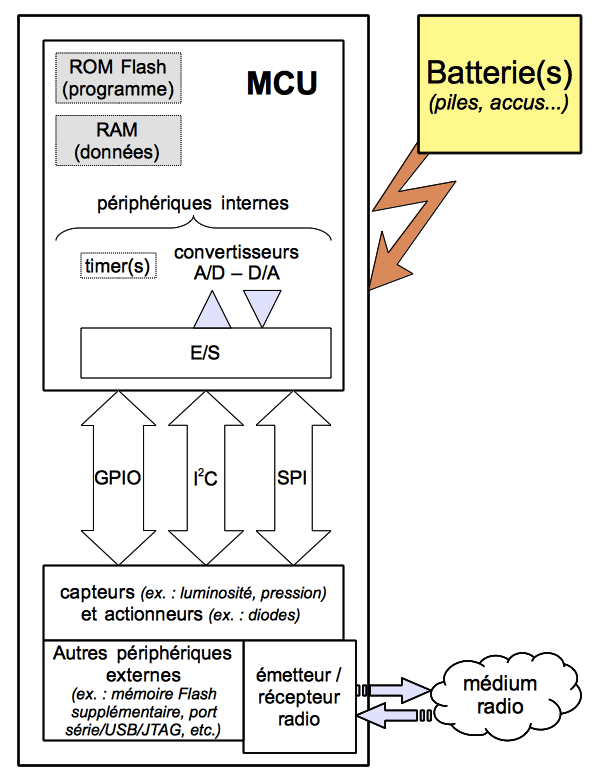
\includegraphics[width=11cm]{images/ch2-structure-mote.png}
\flcaption{Schéma fonctionnel d'une \lang{mote} WSN~/ IoT classique.}
\label{FigStructMote}
\end{figure}

Les motes constituant les \nom{noeuds} des WSN~--- et par extension
de l'IoT~--- sont des appareils extrêmement compacts~: ils sont conçus
autour d'un circuit intégré central regroupant le processeur principal
(CPU) et plusieurs périphériques de base intégrés~: \lang{timers},
convertisseurs A/D et D/A, contrôleurs E/S regroupant des broches à
usage général, des bus SPI et I$^2$C, etc. Ces circuits intégrés
centraux sont appelés \nom{microcontrôleurs} (\nom{MCU}: \lang{Micro
Controller Unit}).

Il faut être bien conscient que ces MCU disposent d'une puissance
de calcul et d'un espace mémoire extrêmement limités~--- non seulement
comparés aux ordinateurs personnels (PC) actuels, mais également en
regard d'appareils mobiles tels que les \lang{smartphones} et les
tablettes. Leur puissance est en fait plutôt comparable, pour les
modèles les moins chers (et donc parmi les plus couramment employés),
à celle des ordinateurs personnels du début des années 1980 (Apple II,
Commodore VIC et 64, Atari 800XL, Amstrad CPC, etc.).

Outre ce MCU central, une \lang{mote} comprend en général seulement
quelques \nom{capteurs} (\lang{``sensors''})~--- et parfois, plus
rarement quelques \nom{actionneurs} (\lang{``actuators''})~--- leur
permettant d'interagir avec leur environnement, en captant et mesurant
des phénomènes physiques environnants~--- température, pression, humidité,
présence d'individus, radioactivité...~; l'ensemble des capteurs
envisageables est quasiment sans limite~--- et en agissant sur
cet environnement pour les \lang{motes} équipées d'actionneurs
(par exemple~: alarme, signaux lumineux, etc.)

De nombreuses \lang{motes} possèdent, pour des raisons pratiques, des
périphériques supplémentaires (externes au MCU)~: on citera par exemple
de la mémoire Flash supplémentaire pour le stockage permanent de
données, ou des ports série~/ USB pour se connecter à un PC~---
principalement à des fins de déboguage.

Une \lang{mote} est bien évidemment équipée d'un émetteur~/
récepteur radio, pour pouvoir communiquer en réseau. Comme dit
ci-dessus, ces appareils sont pour la plupart extrêmement limités
en énergie~; ces émetteurs~/ récepteurs radio utilisent donc un
standard conçu pour consommer très peu d'énergie, en contrepartie
d'un débit très limité (comparable aux premiers modems analogiques du
début des années 1990). La standard spécifiquement conçu dans cette optique
utilisé par la plupart de ces radios est le standard IEEE 802.15.4
\cite{IEEE802154-2011} (ne couvrant que les couches les plus basses
de la pile réseau) que nous décrirons ultérieurement dans le
présent manuscrit en section \vref{SecProto802154}. Notons que
certains MCUs récents, dans un souci d'efficacité et d'intégration,
intègrent directement un émetteur~/ récepteur radio sur la même puce.

Enfin, une \lang{mote} est bien évidemment équipée d'une ou plusieurs
batteries pour son alimentation. Certains modèles de développement~/
déboguage offrent également la possibilité d'être alimentés par une
source d'énergie externe (secteur).

\paragraph{Les middlewares pour WSN.}
\label{ParMiddlewares}

Avant de nous intéresser en détail au fonctionnement technique des couches
de bas niveau des WSN, nous allons très brièvement évoquer un autre
sujet de recherche actif dans le domaine des WSN.

Notons en effet que l'absence de standard officiel pour les WSN au-delà
des deux couches les plus basses fournies par le standard IEEE 802.15.4
(niveaux OSI 1~: PHYsique, et 2~: \lang{Media Access Control}, comme
nous le verrons dans la section \vref{SecProto802154} de l'état
de l'art) a amené à un développement assez anarchique des piles, protocoles
et autres solutions pour les couches plus hautes. À l'heure où nous écrivons
ces lignes, aucune des solutions conçues pour travailler par-dessus les
réseaux 802.15.4 (telles ZigBee, etc.) ne s'est réellement imposée comme
standard, fut-il de fait.

On voit donc, selon les applications prévues pour les différents WSN,
se multiplier des solutions souvent incompatibles dans le déploiement
des différents réseaux de capteurs sans-fil sur le terrain.

Un domaine de recherche dans les WSN est donc la conception de
\emph{``middlewares''} (<<~intergiciels~>>) permettant une interaction
efficace entre tous ces WSN de conception différente et le réseau global
(Internet), pour tenter de faire de l'IoT une réalité tangible, fiable et
donc utilisable industriellement. Un article de référence (\lang{``survey''})
recensait déjà nombre de projets de ce type lors de la décennie précédente
\cite{Middleware-WSN-Survey-2008}.

Nous n'avons au cours de cette thèse malheureusement quasiment pas
eu le temps de nous pencher sur cette problématique, si ce n'est au
début pour travailler très brièvement sur le \lang{middleware} MPIGate
\cite{KR-UbiMob-2013}. Les travaux de la présente thèse concernent,
à l'exception de la publication cité dans la phrase précédente,
uniquement les couches basses des piles réseau des plates-formes
spécialisées pour WSN.


\subsection{Les réseaux de capteurs sans-fil et leur trafic}
\label{SubsecTraficWSN}

Les réseaux de capteurs sans-fil (WSN) sont, comme nous l'avons vu
ci-dessus dans le descriptif des motes, des réseaux à bas débit et
à faible portée, en contrepartie d'une consommation d'énergie très
limitée.

Le trafic réseau est, dans ce genre de réseau, typiquement faible,
avec éventuellement des pointes de débit. Les transmissions entre
noeuds d'un WSN peuvent, par nature, être déclenchées selon trois
modalités différentes~:

\begin{description}

\item[Périodique~:] un noeud capteur analyse son environnement à
intervalles réguliers, en tire une valeur exploitable (par exemple~:
température, pression, etc.), et l'émet sur le réseau à l'aide
de son émetteur~/ récepteur radio. L'intervalle de temps entre
deux mesures~/ émissions est à la discrétion des concepteurs
du WSN et~/ ou des programmeurs de la \lang{mote}.

\item[\'Evènementiel~:] un noeud capteur, lors d'une analyse de
son environnement, capte une valeur~--- ou une variation de valeur~---
anormale ou atypique, et envoie alors un message d'alerte sur le
réseau. Là encore, l'intervalle des valeurs normales, ou le type
d'évènement susceptible de déclencher l'envoi d'une alerte est
à la discrétion des concepteurs du WSN et/ou des programmeurs
de la \lang{mote}.

\item[Par requête~:] un intervenant extérieur au WSN émet, via
la station de base\footnotemark[1] une requête vers une \lang{mote}
donnée, qui y répond par le déclenchement d'un actionneur~--- si
le noeud en est équipé~--- et~/ ou par l'envoi d'une réponse,
correpondant le plus souvent à une valeur analysée par un des
capteurs de la \lang{mote} en question. Ici aussi, la nature des
requêtes et des réponses à y apporter sont à la discrétion des
concepteurs du WSN et/ou des programmeurs de la \lang{mote}.

\footnotetext[1]{La \nom{station de base} est le noeud (\lang{mote}
ou PC ou tout autre appareil connecté) servant de lien entre un
réseau de capteurs sans-fil et le reste de l'Internet~: il s'agit,
pour faire simple, des passerelles de l'Internet des Objets (IoT).
On les nomme également souvent \nom{\lang{``sinks''}}.}

\end{description}

Ces trois modalités ne sont bien évidemment pas exclusives~: un même
WSN peut utiliser les trois types de fonctionnement en fonction des
besoins du moment.

Prenons l'exemple, pour aborder le sujet de l'e-santé qui concerne
cette thèse, d'un WSN destiné à monitorer les signes vitaux d'un
patient sous surveillance (par exemple~: un malade cardiaque)~:

\begin{itemize}

\item En temps normal, les capteurs présents sur le patient relèvent
ses signes vitaux (pulsations cardiaques, pression sanguine, oxymétrie
de pouls, mouvements respiratoires, etc.) de façon régulière et
envoient ainsi (via l'IoT) les résultats à une base de données
spécialisée consultable par les médecins.

\item En cas d'anomalie, (par exemple~: chute de pression sanguine,
ou des pulsations), les capteurs envoient sans attendre un message
d'alerte, qui pourra être relayé aux médecins traitant le patient
ou même, selon la gravité, au SAMU. Un mécanisme d'IoT permettant
d'envoyer des messages (type SMS) à des secouristes présents à
proximité du patient pourrait également être envisagé.

\item En cas de situation critique (par exemple~: fibrillation
cardiaque), les messages d'alerte envoyés plus tôt auront alerté
les services médicaux d'urgence, qui pourront en attendant l'arrivée
physique des secours envoyer (toujours via l'IoT) une requête au WSN
présent sur le patient~: par exemple pour ordonner la mise en action
d'un défibrillateur cardiaque portatif (ou d'un \lang{``pace-maker''})
connecté au WSN porté par le patient.

\end{itemize}

Les possibilités offertes par les WSN~--- ne serait-ce que sur le seul
domaine médical vu dans cet exemple~--- sont donc extrêmement larges.

Il importe toutefois, pour connaître les limites de ces réseaux
de capteurs sans-fil, d'en connaître les spécificités. C'est le
sujet que nous allons maintenant aborder dans la prochaine section.


\subsection{Spécificités des WSN}
\label{SubsecSpecifWSN}

Par rapport aux réseaux traditionnnels, les réseaux de capteurs sans-fil
ont des spécificités, décrites dans la table \vref{TabComparResWSN}.

\begin{table}[!p]
\centering
\begin{tabular}{|p{5.9cm}|p{5.9cm}|}
\hline
\textbf{Réseaux traditionnels}
 & \textbf{Réseaux de capteurs sans-fil} \\
\hline
\emph{Réseaux généralistes~:} conçus pour servir toutes les applications
possibles.
& \emph{Réseaux spécifiques~:} conçus dans un but unique pour servir une
application bien définie.\\
\hline
Les principaux objectifs sont \emph{la performance du réseau et ses
latences}. La consommation d'énergie n'est pas une préoccupation
majeure.
& \emph{L'énergie est une contrainte centrale} dans la conception d'un
réseau de capteurs sans-fil et de chacun de ses noeuds.\\
\hline
Les réseaux sont \emph{conçus et déployés selon des plans pré-déterminés}.
& Le déploiement, la structure des réseaux et l'utilisation des ressources
sont souvent déterminés de manière \nom{ad-hoc} \emph{(sans planification
préalable)}.\\
\hline
Les réseaux et leurs composants opèrent dans des \emph{environnements
contrôlés} et des \emph{conditions environnementales modérées}.
& Les réseaux de capteurs sans-fil opèrent souvent dans des 
\emph{environnements et des conditions hostiles}.\\
\hline
La maintenance et la réparation sont des opérations courantes et
\emph{le réseau et ses composants sont typiquement faciles d'accès.}
& \emph{L'accès physique aux capteurs sans-fil est souvent difficile
voire même impossible}.\\
\hline
\emph{Le coût des composants des réseaux peut être élevé}, selon le
niveau de performances visé.
& \emph{Le coût des capteurs sans-fil doit rester très faible}, d'où le
recours à des composants bon marché aux performances (et parfois à la
fiabilité) limitées.\\
\hline
La défaillance d'un composant du réseau est réglée par \emph{des
opérations de maintenance et de réparation}.
& La défaillance d'un ou plusieurs noeuds est prévisible et
\emph{gérée dans la conception même du réseau}.\\
\hline
La connaissance de l'état global du réseau est typiquement possible
et \emph{la gestion centralisée est possible}.
& La plupart des décisions sont \emph{prises au niveau local sans
intervention d'une gestion centralisée}.\\
\hline
\end{tabular}
\flcaption{Comparaison entre réseaux traditionnels et WSN.
(d'après \cite{LivreDargie2010} table 1.2)}
\label{TabComparResWSN}
\end{table}

\bigskip

Les principaux points déterminants concernant ces spécificités sont les
suivants~:

\begin{itemize}

\item Les capteurs sans-fil sont des appareils dont le coût doit rester
le plus faible possible. Cela influe sur les capacités très limitées
de ces appareils, et aussi potentiellement sur leur fiabilité.

\item Les réseaux de capteurs sans-fil sont généralement des réseaux
\emph{ad-hoc}, c'est-à-dire dont la structure n'est pas planifiée.
Leur mode de fonctionnement est ainsi fondamentalement local, aucune
gestion centralisée n'est en général possible.

\item Les réseaux de capteurs sans-fil sont en général conçus pour
servir une et une seule application donnée au cours de leur existence
(point commun avec l'informatique~/ électronique embarquée). Ils
peuvent être amenés à opérer dans des conditions environnementales
difficiles voire hostiles.

\item Un point commun avec les réseaux traditionnels est la montée
en charge. Un réseau de capteurs sans-fil peut résulter de l'interconnexion
de centaines de PANs, et regrouper ainsi des milliers de \lang{motes}.
De telles tailles de réseau sont rarement atteintes avec les réseaux
sans-fil les plus courants.

\item Les noeuds de ces réseaux pouvant tomber en panne sans pouvoir
être remplacés (défaillance d'un composant, ou d'une batterie non
remplaçable), la structure de tels réseaux doit pouvoir <<~survivre~>>
à ces pannes et les gérer.

\item Ce sont des réseaux sans-fil, dont le médium radio est peu fiable
par nature (par rapport aux réseaux câblés), sujet à la diffusion, et
dont l'état est variable au cours du temps.

\item Enfin, et c'est peut-être le plus important, la consommation
d'énergie est une contrainte extrêmement forte dans les réseaux de capteurs
sans-fil, bien plus que dans n'importe quel autre type de réseau. Cette
contrainte influe directement et lourdement sur la conception des WSN
et de leurs noeuds.

\end{itemize}

\bigskip

Pour répondre à ces différents problèmes, quatre notions liées à
\emph{l'auto-gestion} sont mises en avant dans \cite{LivreDargie2010}
comme caractéristiques désirables pour les WSN~:

\begin{description}

\item[\lang{``Self-organization''},] \nom{auto-organisation~:}
est la capacité d'adapter les paramètres de la configuration du réseau
en fonction de son état et de son environnement.

\item[\lang{``Self-optimization''},] \nom{auto-optimisation~:}
est la capacité de monitorer et d'optimiser l'utilisation des ressources
limitées du réseau.

\item[\lang{``Self-protection''},] \nom{auto-protection~:}
est la capacité de reconnaître les intrusions et attaques et de s'en
protéger.

\item[\lang{``Self-healing''},] \nom{auto-réparation~:}
est la capacité de découvrir, d'identifier la cause et de réagir aux
pannes et défaillances du réseau.

\end{description}

Ces différentes notions amènent à la capacité de ces réseaux de capteurs
sans-fil d'assurer un niveau de service suffisant pour les applications
ayant des contraintes fortes quant à la qualité et le débit de leurs
flux de données. Ce domaine, la \nom{Qualité de Service (QdS)} (\lang{QoS}
en anglais) va être l'objet d'étude de la prochaine section \ref{SecQdS}.

%%%%%%%%%%%%%%%%%%%%%%%%%%%%%%%%%%%%%%%%%%%%%%%%%%%%%%%%%%%%%%%%%%%%%%%%%%%%%

\section{La Qualité de Service (QdS)}
\label{SecQdS}

Note~: cette section est inspirée des informations issues de
\cite{TheseBNefzi} et de \cite{CCMQdS}


\subsection{Notion de QdS}
\label{SubsecDefQdS}

Le terme \nom{QdS} (\nom{<<~Qualité de Service}, en anglais QoS:
\lang{``Quality of Service''}) désigne la capacité à fournir un service,
ici un support de télécommunications, conforme à des exigences de
fonctionnement acceptable à assurer par le fournisseur du service
envers l'utilisateur.

Appliquée aux réseaux à commutation de paquets (réseaux basés sur
l'utilisation de routeurs) la QoS désigne l'aptitude à pouvoir garantir
le non-dépassement d'un niveau acceptable de baisse de qualité, défini
contractuellement, pour un usage donné (voix sur IP, vidéo-conférence, etc.).

En effet, contrairement aux réseaux à commutation de circuits, tels que
le réseau téléphonique commuté, où un circuit de communication est dédié
pendant toute la durée de la communication, il est impossible sur Internet
de prédire le chemin emprunté par les différents paquets.

Cette incertitude est encore plus forte sur les réseaux sans-fil,
où le médium radio lui-même est sujet à la diffusion, dont l'état
et l'encombrement peuvent varier fortement et rapidement au cours
du temps. Ce médium est, comparé aux câbles des réseaux informatiques
<<~classiques~>>, bien moins fiable.

Ainsi, rien ne garantit qu'une communication nécessitant une régularité
du débit pourra avoir lieu sans encombre. C'est pourquoi il existe des
mécanismes, dits mécanismes de QoS, permettant de différencier les
différents flux réseau et réserver une partie de la bande passante
pour ceux ayant une importance particulière.

Plus formellement, la recommandation E.800 de septembre~2008 de l'Union
Internationale des Télécommunications (UIT) définit la QdS comme étant
<<~l'ensemble des caractéristiques d'un service de télécommunication qui
lui permerrent de satisfaire aux besoins explicites et aux besoins
implicites de l'utilisateur du service~>>~; une caractéristique étant
définie comme une <<~propriété (qualitative ou quantitative) qui aide
à faire la distinction entre les individus d'une population donnée~>>.

En termes pratiques, une caractéristique du standard E.800 de l'UIT
correspond à un critère de QdS. Le but à atteindre étant d'assurer
une valeur minimale en-deça de laquelle ne pas tomber pour respecter
un contrat de qualité avec l'utilisateur.

\newpage


\subsection{Critères de QdS}
\label{SubsecCritQdS}

Les principaux critères permettant d'apprécier la qualité de service
sont les suivants~:

\begin{description}

\item[Perte de paquets] (en anglais \lang{packet loss})~: elle
correspond à la non-délivrance (perte) de paquets de données, la plupart
du temps dûe à un encombrement du réseau.

\item[Débit] (en anglais \lang{bandwith})~--- encore appelée \nom{bande
passante}~--- il définit le volume maximal d'information (bits) pouvant
transiter par unité de temps.

\item[Latence, délai, ou temps de réponse] (en anglais \lang{delay})~:
elle caractérise le retard entre l'émission et la réception d'un
paquet de données.

\item[Gigue] (en anglais \lang{jitter})~: elle représente la fluctuation
du signal numérique, dans le temps ou en phase.

\item[Déséquencement] (en anglais \lang{desequencing})~: correspond à
une modification de l'ordre d'arrivée des paquets.

\end{description}

Le rôle d'une politique ou d'un mécanisme de QdS est de toujours garder
une valeur acceptable (égale ou supérieure à une valeur-seuil de
qualité minimale) pour ces différents critères.

(\`A noter qu'à côté de ces principaux critères de QdS, d'autres peuvent
être pris en compte, comme par exemple la durée de vie de chaque noeud,
le MTBF, le respect du coût, etc.)

\subsection{Stratégies d'assurance de la QdS}
\label{SubsecStratQdS}

Les stratégies classiques appiquées pour assurer une QdS optimale
peuvent se diviser en deux grandes catégories~:

\begin{itemize}

\item Les méthodes de contrôle \lang{a priori} ou \emph{préventives}
du trafic réseau que sont~:
  \begin{itemize}
  \item les politiques de gestion de files d'attente, ou ordonnancement,
        permettant la mise en place de la différentiation de service~;
  \item le lissage (ou mise en forme) du trafic, consistant à contrôler
        le volume du trafic entrant dans le réseau, la plupart du temps
        selon les méthodes du seau percé ou du seau à jetons~;
  \item le contrôle du trafic, et sa variante extrême, le contrôle
        d'admission, consistant à refuser le trafic entrant en
        fonction de certains critères.
  \end{itemize}

\item Les méthodes de contrôle \lang{a posteriori} ou \emph{réactives}
du trafic réseau~:
  \begin{itemize}
  \item le contrôle de congestion, acceptant tout le trafic arrivant
        en conditions normales, et diminuant le débit ou supprimant
        des paquets lors de la survenue d'une congestion~; le mécanisme
        de fenêtre de congestion de TCP~/ IP fait partie de ces méthodes~;
  \item le choix dynamique des routes, pour assurer la meilleure QdS
        possible en fonction de l'état courant d'un réseau~: ce
        mécanisme dépend du protocole de routage de la pile réseau.
  \end{itemize}

\end{itemize}

D'une façon générale, les méthodes de contrôle réactives semblent se
montrer mieux adaptées aux réseaux sans-fil, notamment aux WSN, les
méthodes proactives s'adaptant mal au médium radio et ses caractéristiques.


\subsection{Niveaux de service}
\label{SubsecNivQds}

Le terme \nom{niveau de service} (en anglais \lang{Service level}) définit
le niveau d'exigence pour la capacité d'un réseau à fournir un service
point à point ou de bout en bout avec un trafic donné. On définit
généralement trois niveaux de QdS :

\begin{description}

\item[Service garanti] (en anglais \lang{guaranteed service} ou 
\lang{hard QoS}), consistant à réserver des ressources réseau pour certains
types de flux. Le principal mécanisme utilisé pour obtenir un tel niveau
de service est RSVP (\lang{Resource reSerVation Protocol}, en français
<<~Protocole de réservation de ressources~>>).

\item[Service différencié] (en anglais \lang{differenciated service} ou
\lang{soft QoS}), permettant de définir des niveaux de priorité aux
différents flux réseau sans toutefois fournir une garantie stricte.

\item[Meilleur effort] (en anglais \lang{best effort}), ne fournissant
aucune différenciation entre plusieurs flux réseaux et ne permettant
aucune garantie. Ce niveau de service est ainsi parfois appelé
(abusivement) \lang{lack of QoS}.

\end{description}


\subsection{QdS dans les réseaux de capteurs sans-fil}
\label{SubsecQdsWSN}

Les données venant d'être exposées jusqu'ici dans la présente section
\ref{SecQdS} concernent la QdS en général~: elles s'appliquent à tous
les types de réseaux.

Pour les réseaux de capteurs sans-fil, la nature même du réseau, avec
des noeuds aux capacités très limitées, une contrainte énergétique
très forte, un médium radio non-fiable, et une possibilité de défaillance
de noeuds, rend les notions de service garanti ou différencié impossibles
à atteindre. \emph{La Qualité de Service, dans le domaine des WSN,
est donc quasiment toujours une garantie du type \lang{``best effort''}}.

Concernant les critères de QdS importants et gérés au niveau des
couches MAC~/ RDC des WSN, on s'intéresse principalement au
\emph{taux de perte de paquets} et au \emph{délais de transmission}.
Les autres critères étant soit définis par les standards gérant
le médium radio~--- par exemple~: le débit (théorique) de 250~Kbit/s
pour le standard 802.15.4 sur la bande 2,4 GHz~---~; soit dépendants
de conditions externes sur lesquelles aucune intervention n'est possible
(gigue, débit réel diminué par des interférences radio)~; soit réglés
par les couches supérieures des piles réseau (déséquencement des paquets).

Enfin, le caractère extrêmement contraignant de la limitation énergétique
fait de cette \emph{obligation d'économie d'énergie un critère à part
entière de la QdS}~--- bien que celui-ci soit contradictoire avec les
autres critères de QdS. En effet, les \lang{motes} étant souvent dans
des situations où le changement de batterie est difficile ou même impossible,
conserver la batterie opérationnelle le plus longtemps possible revient à
maintenir le noeud correspondant <<~en vie~>> le plus longtemps possible.
Une \lang{mote} à cours d'énergie est en effet souvent une \lang{mote}
perdue définitivement, donc une perte de fonctionnalité~--- potentiellement
sévère~--- pour le WSN correspondant.

En résumé, on peut dire que pour les WSN, le lien entre Qualité de Service
<<~fonctionnelle~>> (bande passante, fiabilité et rapidité des transmissions)
et économie d'énergie est tout à la fois contradictoire, indissociable
et crucial. L'optimisation de la QdS revient ainsi toujours à trouver
\emph{le meilleur compromis, l'équilibre optimal} entre tous les facteurs
cités dans cette présente section \ref{SubsecQdsWSN}, en fonction de
l'application voulue.

\bigskip

Après toutes ces définitions techniques, nous allons maintenant dans la
section \ref{SecAppWSN} suivante passer en revue les différents domaines
d'applications des WSN. Comme nous allons le voir, ceux-ci sont nombreux
et variés.

%%%%%%%%%%%%%%%%%%%%%%%%%%%%%%%%%%%%%%%%%%%%%%%%%%%%%%%%%%%%%%%%%%%%%%%%%%%%%

\section{Applications des WSN (et de l'IoT)}
\label{SecAppWSN}

Akyildiz et Vuran, dans leur livre \cite{LivreAkyildiz2010}, considèrent
cinq grands types d'applications aux WSN (voir figure
\vref{FigAppWSNAkyildiz})~:

\begin{figure}[hbt]
\centering
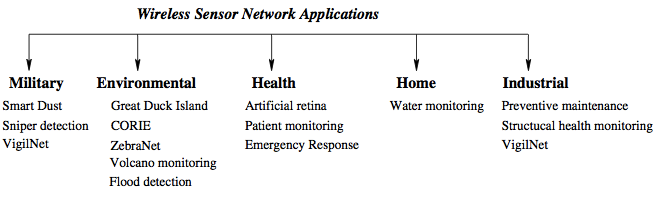
\includegraphics[width=12.5cm]{images/ch2-app-wsn.png}
\flcaption{Principales catégories d'application des réseaux de
capteurs sans-fil.
Source~: \cite{LivreAkyildiz2010}, figure 2.1.}
\label{FigAppWSNAkyildiz}
\end{figure}

\begin{description}

\item[Applications militaires~:] les buts sont multiples, comme le contrôle
des forces alliées, de leur équipement et de leurs munitions, la surveillance
du champ de bataille, la reconnaissance de l'ennemi et du terrain,
l'évaluation des dégâts, ou la détection d'attaques non conventionnelles.
Plusieurs exemples sont cités dans \cite{LivreAkyildiz2010}~: le projet
\lang{Smart Dust} du DARPA (un pionnier dans les WSN), ou un système de
détection de \lang{sniper} \footnotemark[2].
\footnotetext[2]{Démontrations vidéos sur cette page Web~:
\texttt{http://bbn.com/boomerang}}

\item[Applications industrielles~:] ici aussi, les applications sont
nombreuses~: la supervision des processus de fabrication et la vérification
de la qualité de production, la localisation et la surveillance de
l'équipement industriel, la maintenance préventive des usines (surtout de
grande taille) et des conditions de travail ou d'opération du matériel
industriel, etc. Un exemple cité dans \cite{LivreAkyildiz2010} est
le projet FabApp \cite{FabApp}, dont le but est d'évaluer les vibrations
du matériel industriel lors de son fonctionnement pour prévenir
pannes et accidents (tant dans une usine de fabrication de semi-conducteurs
que dans un pétrolier).\\
On pourra également citer des applications de contrôle de l'état structurel
des bâtiments, comme par exemple la surveillance active du \lang{Golden Gate
Bridge} (San Francisco) \cite{AppGoldenGate}.\\
Citons aussi l'assistance au domaine minier~: l'objectif étant de détecter
les évènements dangereux pour les mineurs (poches de gaz, responsables
de <<~coups de grisou~>>) ainsi que de quantifier les émissions de méthane
produites par les mines de charbon (le méthane étant un gaz à effet de
serre, celui-ci influe sur le changement climatique actuel).

\item[Applications environnementales~:] de nombreux projets sont
réalisables, comme le suivi des mouvements d'animaux, la détection de feux
de forêts ou d'inondations, la recherche météorologique ou géophysique,
l'étude de la pollution, etc. Plusieurs exemples sont cités dans
\cite{LivreAkyildiz2010}, parmi lesquels~: \lang{ZebraNet} \cite{ZebraNet}
un système de surveillance au long cours de la population de zèbres,
déployé au Kenya. Autre exemple~: un système de surveillance des volcans
\cite{VolcansWSN}~--- également cité dans \cite{LivreDargie2010}~---
le but étant ici de détecter à l'avance les signes avant-coureurs des
éruptions, pour mieux prévenir celles-ci, ou d'étudier le fonctionnement
de volcans sous-marins, pour mieux comprendre les phénomènes d'activité
volcanique. On peut aussi citer un système de détection précoce
d'inondations dans les pays en voie de développement \cite{FloodDetect}.\\
Les réseaux de capteurs sans-fil servent également à l'agriculture de
précision, en permettant d'analyser précisément l'état des sols, afin de
mieux utiliser les ressources à utiliser (eau, engrais, pesticides,
herbicides) pour optimiser les récoltes. Plusieurs projets prototypes
ont déjà été déployés dans ce but.\\
L'environnement urbain peut également en bénéficier, par exemple par des
applications de contrôle actif du trafic routier aux \'Etats-Unis
\cite{ControleTrafic}, ou encore le projet PipeNet \cite{PipeNet}
mis en place dans de nombreuses villes américaines pour monitorer
les réseaux d'égoûts.

\item[Applications à la santé~:] le domaine de la santé fait partie du
contexte de la présente thèse, et nous y reviendrons donc plus longuement
dans une section suivante (section \vref{SubsecSanteWSN}).

\item[Applications domotiques~:] On cite dans \cite{LivreAkyildiz2010}
un système nommé NAWMS \cite{NAWMS} destiné à détecter les gaspillages
d'eau et leur origine précise, afin d'en informer les usagers pour
les aider à réduire leur facture d'eau.

\end{description}

En étudiant les applications des WSN et de l'IoT citées dans
\cite{LivreDargie2010} et \cite{LivreAkyildiz2010}, on voit que ces
applications ne manquent pas, et sont appelées à continuer à se développer
de façon exponentielle.

\newpage

Nous allons maintenant dans la section \ref{SecContexte} suivante
nous focaliser sur le contexte de la présente thèse.

Ce contexte est celui du domaine d'application de la santé pour les WSN.
Nous y étudierons tout particulièrement le projet LAR (\lang{``Living
Assistant Robot''}), dont cette thèse fait partie, dans la section
\vref{SubsecLAR}.

%%%%%%%%%%%%%%%%%%%%%%%%%%%%%%%%%%%%%%%%%%%%%%%%%%%%%%%%%%%%%%%%%%%%%%%%%%%%%

\section{Contexte}
\label{SecContexte}


\subsection{Applications d'e-santé des WSN}
\label{SubsecSanteWSN}

L'utilisation des réseaux de capteurs sans-fil pour des applications
dans le domaine de la santé est un domaine déjà bien établi et très
actif~: les PAN (\lang{Personal Area Network}) dédiés à être installés
sur un patient~--- par exemple pour suivre son état de santé~--- sont
même désignés par un acronyme spécifique~: \nom{BAN} \emph{(\lang{``Body
Area Network''})}.

Les applications des WSN au domaine de la santé sont également, comme dans
les autres domaines, très nombreuses et variées~: un article complet
de référence \cite{WSN-HealthCare-Survey-2010} recensait en 2010 les
nombreux projets d'exploitation des réseaux de capteurs sans-fil liés
au domaine de la santé.

Parmi les projets les plus ambitieux, les deux livres de
\cite{LivreDargie2010} et de \cite{LivreAkyildiz2010} citent tous deux des
projets de rétines artificielles \cite{RetineArtificielle}
\cite{RetineArtificielle2} combinant une caméra CCD externe couplée à des
nano-noeuds sans-fil implantés \emph{in vivo} sur la rétine du patient.
Ces projets visent à apporter une solution à des maladies actuellement
incurables, comme la DMLA (Dégénérescence Maculaire Liée à l'Âge) ou
la rétinite pigmentaire (maladie génétique).

Sans aller jusqu'à des projets aussi avancés technologiquements (et
organiquement invasifs) de nombreux projets de surveillance à domicile
de patients fragiles et de réponse aux cas d'urgence sont actuellement
mis en place.

Rappelons notamment l'existence du projet \nom{d'informatique située},
consistant en une plate-forme d'<<~appartement intelligent pour l'assistance
à la personne~>> \cite{AppartIntelligent}, utilisant intensivement les WSN,
que l'on peut classer à la fois dans les applications domotiques et les
applications à la santé. Ce projet, hébergé au LORIA~/ INRIA Nancy Grand-Est,
implique directement (entre autres) notre équipe~--- Madynes~---, et l'un
des encadrants de la présente thèse~--- Y.-Q. Song.


\subsection{Le projet LAR}
\label{SubsecLAR}

Un autre de ces projets fait également usage des WSN, combinant aussi~---
comme nous l'avons dit auparavant au chapitre \ref{ChIntro}~--- aspect
domotique et aspect santé, est le \nom{projet LAR} (\lang{``Living Assistant
Robot''}), dont la présente thèse fait partie.

\newpage

Le projet LAR a pour objectif d'aider au maintien à domicile des personnes
âgées et~/ ou dépendantes, et de tenter de retarder le plus possible le
moment où ces dernières doivent être placées en institutions spécialisées,
ce qui représente un coût financier et surtout humain considérable.

Dans ce but, le projet vise à fournir des outils de suivi à domicile
de la personne dépendante et de son activité, de développer pour cela
des outils de perception, de modélisation de l'activité humaine,
et d'interaction avec la personne. Comme le nom du projet l'indique,
il est question de fournir (du moins dans le cas les plus lourds)
un robot d'assistance spécialement conçu par le projet~; mais une
grande partie du travail fourni (détection de présence, de mouvement,
de chutes, etc.) sera fourni par un ou plusieurs WSN installés chez
le patient, le robot étant également porteur de capteurs et actionneurs
et donc membre à part entière de ce(s) WSN. Ces WSN sont également reliés
à l'IoT, les données médicales recueillies étant destinées à être
stockées dans des bases médicales spécialisées, accessibles de façon
sécurisée aux personnels de soins (médecins, infirmiers, etc.).

Le principe central du projet LAR est la mise en {\oe}uvre d'un écosystème
modulaire de services (comme nous venons de le voir~: capteurs de données
de toutes natures, robots, mais aussi services à la personne, etc.),
lesquels services opèrent au sein d'une architecture orientée services
(\lang{``Service Oriented Architecture''} ou \nom{SOA}) centrée sur un
orchestrateur (alias \lang{``Enterprise Message Bus''}) Microsoft BizTalk.

L'un des objectifs fondamentaux du projet est de commercialiser ce
service au coût le plus faible possible, afin de le rendre accessible
au plus grand nombre~; c'est pourquoi le recours à des WSN (avec leurs
\lang{motes} à faible coût) est un point clé du programme. L'une des
idées directrices du projet est de rendre l'offre modulaire, et de ne
fournir que les services nécessaires à l'état courant du patient~:
les cas les plus légers n'auront ainsi que l'installation d'un WSN
<<~léger~>> et peu intrusif à leur domicile, l'évolution de l'état
du patient pouvant ensuite amener à recourir à des modules
supplémentaires~; le robot étant l'élément le plus évolué mais aussi
le plus coûteux.

Plusieurs partenaires académiques et industriels sont impliqués dans
ce projet~: la partie académique est représentée par le LORIA~/ INRIA
Nancy Grand-Est en l'équipe Madynes (dont nous faisons partie) pour les
WSN, et l'équipe Larsen~--- anciennement Maia~--- pour la partie robotique
et reconnaissance des mouvements~; les partenaires industriels sont
Diatelic (pour la gestion de la base de données médicales et son accès
sécurisé), Robosoft S.A. (pour la conception et la fabrication du robot),
et le Pôle Innovation du Crédit Agricole S.A. (qui coordonne le projet).
Tous ces partenaires ont formé un consortium~--- dont le Crédit Agricole
a pris la tête~--- pour répondre à l'appel d'offres <<~e-santé~>> lancé
en 2011 par la DGCIS~--- depuis devenue DGE (Direction Générale des
Entreprises)~---, lequel consortium a remporté l'appel et ainsi fondé
le projet LAR. Le contrat correspondant a été signé en 2012, et le projet
LAR a été financé par la Banque Publique d'Investissement (BPIFrance).

%%%%%%%%%%%%%%%%%%%%%%%%%%%%%%%%%%%%%%%%%%%%%%%%%%%%%%%%%%%%%%%%%%%%%%%%%%%%%

\section{Problématique}
\label{SecProblematique}


\subsection{Exposé de la problématique}
\label{SubsecExposeProblematique}

Dans le domaine des réseaux de capteurs sans-fil, les piles réseau
spécialisées constituent un domaine de recherche très actif depuis
maintenant une quinzaine d'années. On citera actuellement, par exemple
dans le domaine des couches hautes, les protocoles de routage (RPL et ses
nombreuses variantes et évolutions), ou encore l'activité actuelle autour
des CCN (\lang{``Content-Centric Networks''}).

Pour les couches basses, de nombreux travaux de recherche ont également
été effectués sur les protocoles MAC (la couche MAC représentant le
niveau 2 dans le modèle OSI), pour suppléer le protocole du
standard 802.15.4 et ses limitations, comme nous le verrons au
chapitre \vref{ChEtatArt}. Toutefois, beaucoup de ces études se
sont principalement consacrées à l'étude théorique de ces protocoles,
se contentant souvent~--- à des fins de tests~--- de simulations
puremement théoriques (avec des outils comme OPNET, ns-3, OMNeT++, voire
même MATLAB), ou au mieux par des émulations de \lang{motes} virtuelles
(avec des outils comme TOSSIM \cite{TOSSIM} ou Cooja \cite{Cooja}).

L'implantation de ces couches basses, dans les plates-formes logicielles
réelles~--- c'est à dire les systèmes d'exploitation dédiés aux réseaux de
capteurs sans-fil~--- n'a pas fait l'objet d'un effort de recherche poussé
et systématique. Le principal but était de minimiser la consommation
d'énergie de ces couches basses, généralement en ayant recours aux
protocoles et aux implantations les plus simples possibles.

L'un des seuls efforts remarquables de conception et d'implantation
dans ce domaine, le protocole ContikiMAC~--- développé spécifiquement
pour la plate-forme logicielle Contiki OS~--- a ainsi comblé un manque,
et est devenu le standard de fait, du moins dans la littérature sur le
domaine des réseaux de capteurs sans-fil. Depuis, on ne peut qu'observer
un certain \lang{statu quo} dans ce domaine. Si de nombreux protocoles
MAC à hautes performances ont été conçus (comme nous le verrons dans
la section \vref{SecProtoMAC} de l'état de l'art), aucun d'entre
eux n'a été implanté et largement diffusé avec un OS spécialisé
comme l'est ContikiMAC.


\subsection{Stratégie préconisée}
\label{SubsecStrategieThese}

\subsubsection{Besoins identifiés}
\label{ParBesoins}

Pour avancer dans ce domaine, et notamment pouvoir exploiter les
nouvelles \lang{motes} plus puissantes~--- par exemple celles basées
sur des microcontrôleurs à base ARM Cortex-M~--- rencontrées de plus
en plus souvent (en sus des plates-formes classiques à base MSP430
ou AVR), nous voyons plusieurs besoins à combler~:

\begin{enumerate}

\item \emph{Faire évoluer les plates-formes logicielles (OS) spécialisées
dans les réseaux de capteurs sans-fil, en leur ajoutant des
fonctionnalités nécessaires au développement de piles réseau plus
performantes.}\\
La programmation sans OS ni plate-forme d'aucune sorte (programmation
\lang{``bare metal''}) nous semble à proscrire, car les logiciels ainsi
créés ne sont nullement portables, et doivent être réécrits à chaque
changement de matériel, lequel dans ce domaine (comme dans toute
l'électronique et l'informatique) évolue très vite.\\
L'utilisation d'une plate-forme logicielle facilite aussi la programmation
d'applications, ainsi que les travaux d'évaluation et de comparaison.

\item \emph{Expérimenter, de façon intensive et approfondie, ces
plates-formes logicielles spécialisées et leurs piles réseau} afin de les
optimiser et de les fiabiliser, tout spécialement leurs couches basses.

\item \emph{Tester le comportement et la résilience de ces piles réseau
spécialisées (et notamment de leurs couches basses) face à des charges
réseau intenses.} En effet, la plupart des réseaux de capteurs sans-fil
actuels sont conçus pour gérer des trafics faibles à modérés. \emph{Lors de
situations exceptionnelles~--- tout spécialement dans le domaine médical~---
on peut imaginer que ces WSN puissent avoir à gérer des trafics intenses,
que ce soit de façon ponctuelle (par exemple~: gestion d'un patient
à domicile en situation d'urgence vitale) ou continue (comme dans une
maison médicalisée ou un hôpital où de nombreux WSN traiteront constamment
et de façon concurrente de fortes quantités de données).} Nous souhaitons
dans cette thèse évaluer, et si nécessaire améliorer et optimiser,
le fonctionnement des couches basses~--- niveaux 1 et surtout 2 du modèle
OSI~--- de ces piles réseau spécialisées face à de telles situations.

\end{enumerate}

Nous nous proposons donc, dans cette thèse, de nous pencher sur les
implantations de ces couches basses, au sein d'un ou plusieurs
systèmes d'exploitation spécialisés offrant les fonctionnalités
nécessaires, et de les optimiser. Nous souhaitons pour cela utiliser
l'approche décrite dans la section \ref{ParApproche} suivante.

\subsubsection{Approche mise en {\oe}uvre}
\label{ParApproche}

Lorsque l'on programme les appareils miniatures qui constituent les
noeuds des WSN, il est nécessaire de s'adapter aux spécificités et aux
limitations de ces appareils. Ainsi, outre leur puissance très limitée,
le principal objectif lorsque l'on programme des \lang{motes} est de
réduire autant que possible leur consommation énergétique. Le but
est de faire durer leur(s) batterie(s) aussi longtemps que possible,
pour des raisons économiques mais également pratiques~: il est parfois
difficile~--- et même quasiment impossible~--- de changer les batteries
de certaines de ces \lang{motes}, à cause de leur localisation
(par exemple~: en haut d'immeubles, sous des routes, etc).

De tous les différents composants constituant une \lang{mote}, l'élément
le plus consommateur d'énergie est, de loin, l'émetteur~/ récepteur
radio (comparer, par exemple, les consommations énergétiques d'un émetteur~/
récepteur radio comme le TI CC2420 \cite{DSCC2420} et d'un microcontrôleur
comme le MSP430F1611 \cite{DSMSP430F1611}, qui sont les deux principaux
composants de la famille répandue de motes que sont les TelosB~/ SkyMotes
\cite{DSTelosB}). En conséquence, pour limiter la consommation énergétique
de ces appareils, un premier point-clé est d'utiliser cet émetteur~/
récepteur radio uniquement quand cela est nécessaire, en le gardant
éteint~--- ou en mode <<~sommeil~>> aussi souvent que possible.
L'élément logiciel responsable de contrôler cet émetteur~/ récepteur
radio de façon adéquate est le niveau 2 de la pile réseau logicielle,
constituant les couches \nom{MAC} (\lang{Media Access Control}) et
\nom{RDC} (\lang{Radio Duty Cycle}). Cela implique aussi le plus
souvent d'intervenir sur la couche de niveau 1~: la couche \nom{PHY}
ou physique, c'est-à-dire le pilote de l'émetteur~/ récepteur radio,
afin que ce dernier fournisse les fonctionnalités nécessaires aux
couches supérieures (notamment la couche MAC~/ RDC) de la façon
la plus efficace possible.

\emph{Une stratégie efficace d'économie d'énergie pour les \lang{motes}
repose ainsi sur la recherche du meilleur compromis entre d'une part
la réduction de la fraction de temps durant laquelle la radio est active
(\lang{``duty cycle''}), et d'autre part le maintien de la plus haute
efficacité possible du réseau sans-fil (QdS). Ce compromis s'atteint
en développant de nouveaux protocoles MAC~/ RDC <<~intelligents~>>,
s'adaptant dynamiquement et automatiquement au trafic réseau en cours
d'exécution.}

Pour implanter de nouveaux protocoles MAC~/ RDC à hautes performances,
il est nécessaire de pouvoir réagir aux évènements~--- par exemple~:
expirations de délais ou arrivées de paquets, prenant souvent au niveau
de la programmation la forme d'interruptions~--- avec une bonne réactivité
(latence la plus faible possible) et avec flexibilité. De tels protocoles
reposent sur un \lang{timing} précis pour assurer une synchronisation
efficace entre les différentes \lang{motes} et autres appareils équipés
de radio amenés à faire partie des PANs, permettant ainsi de faire
fonctionner les émetteurs~/ recepteurs radio de ces appareils
\emph{uniquement} lorsque cela est nécessaire.

Le deuxième élément le plus consommateur d'énergie dans une \lang{mote},
après l'émetteur~/ récepteur radio, est le microcontrôleur (MCU) au coeur
de cette \lang{mote}. Tous les MCUs actuels offrent des <<~modes à basse
consommation d'énergie~>>, consistant à <<~éteindre~>> à la demande les
différents circuits intégrés au MCU, à commencer par le coeur CPU lui-même.
Le principal moyen de minimiser la consommation d'énergie d'un MCU est ainsi
de désactiver ses fonctionnalités selon les besoins du moment, en ne les
réactivant que quand elles sont nécessaires au fonctionnement courant de
l'application~: cela revient effectivement à mettre le MCU en sommeil
aussi souvent et aussi complètement que possible, tout en continuant
d'exécuter de façon optimale l'application voulue.

Rappelons toutefois que le contexte de notre thèse (applications médicales)
nous poussera toujours à priviligier d'abord la QdS, même si l'optimisation
de la consommation d'énergie doit en souffrir. Cette approche est constante
dans ce travail de thèse~; elle est notamment ce qui nous pousse à tester
les couches basses des piles réseau en situation de trafic intense.
 
Dans les deux cas, pour la gestion de l'émetteur~/ récepteur radio comme
pour celle du MCU, il est nécessaire de pouvoir utiliser les \lang{timers}
matériels et les interruptions de façon optimale, pour pouvoir mettre en
sommeil et réactiver ces circuits de manière efficace afin d'atteindre
le meilleur compromis entre QdS et économies d'énergie, là encore
de façon dynamique et automatique.

\newpage

Être capable d'utiliser les \lang{timers} et les interruptions de façon
efficace et avec un minimum de difficultés implique l'utilisation d'un
système d'exploitation (OS) spécialisé dans les capteurs sans-fil~--- une
plate-forme logicielle adaptée~--- qui nous offrira en outre les bénéfices
de la portabilité de nos applications, et des fonctionnalités
multitâches facilitant la programmation (revoir le premier point abordé
plus haut dans la section \vref{ParBesoins}).

La recherche de cette plate-forme logicielle la mieux adaptée à nos
besoins~--- outre une section consacrée aux OS spécialisés dans le chapitre
sur l'état de l'art (section \vref{SecOSWSN})~--- fera l'objet
d'un chapitre dédié (chapitre \ref{ChPFLogicielles}).

Mais auparavant, nous allons nous pencher sur l'état de l'art concernant les
domaines concernés par cette thèse dans le chapitre \ref{ChEtatArt} suivant.


%%%%%%%%%%%%%%%%%%%%%%%%%%%%%%%%%%%%%%%%%%%%%%%%%%%%%%%%%%%%%%%%%%%%%%%%%%%%%
%%%              FIN DU CHAPITRE "CONTEXTE ET PROBLÉMATIQUE"              %%%
%%%%%%%%%%%%%%%%%%%%%%%%%%%%%%%%%%%%%%%%%%%%%%%%%%%%%%%%%%%%%%%%%%%%%%%%%%%%%



